%\documentclass[12pt,a4paper]{article}
%\usepackage[english]{babel}
%\usepackage{amssymb}
%\usepackage[dvips]{graphicx}
%\setlength{\textwidth}{6.5in}
%\setlength{\oddsidemargin}{0.0in}
%\setlength{\evensidemargin}{0.0in} 
%\setlength{\textheight}{9.5in}
%\addtolength{\topmargin}{-0.8in}

\documentclass[12pt]{article} % `article' with A4 paper size option
\usepackage{amsmath,amssymb,color,amscd,wrapfig}
\usepackage[utf8]{inputenc}

\ifx\pdfoutput\undefined
\usepackage{graphicx}
\else
\usepackage[pdftex]{graphicx}
\fi

\marginparwidth 40pt
\textwidth=140mm
\textheight=206mm


\title{ Denkaufgaben für Kinder von 5 bis 15}

\author{V.\,I.~Arnold
\vspace*{2cm}\\ 
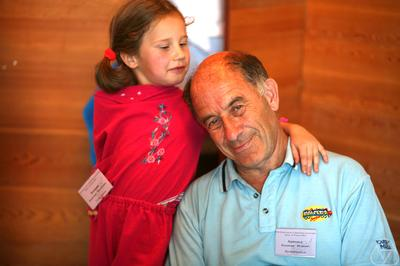
\includegraphics[width=12cm]{photo-arnold_small}
}

\date{}
\begin{document}
%\sloppy
\def\eps{\varepsilon}
%%\vskip7cm
\maketitle
\thispagestyle{empty}

\newpage 
\setcounter{page}{1}
\begin{abstract}

Dieses Sammlung enthält 77 Rätsel für die Förderung und Entwicklung einer Kultur des Denkens. Die Rätsel wurden von dem Autor ausgewählt oder erfunden. Die meisten darunter erfordern keine besonderen Vorkenntnisse jenseits einer allgemeinen Schulbildung, aber manche unter ihnen könnten auch einen Universitätsprofessor oder eine Universitätsprofessorin herausfordern. 

Das Buch richtet sich an Schülerinnen und Schüler, Studentinnen und Studenten, Lehrerinnen und Lehrer und Eltern. Er richtet sich, in anderen Worten, an all jene, die eine Kultur des Denkens als wesentlichen Teil der Persönlichkeitsentwicklung ansehen.

\end{abstract}

\newpage

Ich fing an diese Rätsel aufzuschreiben, nachdem mich im Frühling 2004 russische Pariser baten, ihre Kindern in der Förderung einer Kultur des Denkens zu unterstützen, so wie sie in Russland Tradition hat.

Ich bin fest überzeugt, dass diese Kultur des Denkens schon in der frühen Kindheit besonders durch selbstständiges Tüfteln bei Fragestellungen unterstützt wird, die einfach zu begreifen, aber dafür nicht unbedingt leicht sind. Solche Fragen findet der Leser in dieser Sammlung, besonders empfehle ich Aufgaben Nummer 1, 3 und 13.

Meine lange Erfahrung hat mir gezeigt, dass oft die "schwächeren" Schülerinnen und Schüler solche Fragen besser beantworten können als akademisch erfolgreichere Kinder. Denn für ihr Überleben auf der hinteren Schulbank handeln sie wie Figaro, der “mehr Kenntnisse und Berechnung gebrauchen mußte, bloß um zu bestehen, als man seit hundert Jahren gebraucht hat, um ganz Spanien zu regieren”. Währenddessen verliert sich die gute Schülerin oder der gute Schüler zu oft in der Frage, was man denn jetzt zusammen multiplizieren muss. 

Ich habe auch feststellen können, dass ein fünfjähriges Kind solche Rätsel oft besser lösen kann als routine-verdorbene Schülerinnen und Schüler, die wiederum besser als ambiziöse Universitätsstudierende (die schlechtesten Löser solcher Aufgaben sind auf jeden Fall Nobel- und Fields-Preisträgerinnen und -träger).


\ 

\vspace{0pt plus 12pt}
\centerline{*\quad *\quad*}
\vspace{.4\baselineskip}

\

%\newpage
\noindent{\bf 1.} 

Masha fehlen sieben Kopeken, um ein Lesebuch zu kaufen, und Misha fehlt eine Kopeke. Auch wenn sie ihr Geld zusammen tun, um das Buch gemeinsam zu kaufen, fehlt ihnen immer noch Geld. Wie viel kostet das Buch? 
\newline\newline\quad

{\bf 2.} 
Eine Flasche mit Korken kostet 10 Kopeken. Die Flasche alleine kostet 9 Kopeken mehr als der Korken. Wie viel kostet die Flasche ohne Korken?

\newline\newline{}\quad
{\bf 3.} 

Ein Ziegel wiegt soviel wie ein Pfund und ein halber Ziegel. Was ist das Gewicht eines Ziegels? 
\newline\newline\quad
{\bf 4.} 

Ein Löffel Wein wird von einem Fass in ein (nicht volles) Glas Tee gegossen und verrührt. Danach wird ein Löffel dieser jetzt gemischten Flüssigkeit aus dem Glas zurück in das Fass gefüllt. Also ist in beiden Behältern jeweils etwas einer fremden Flüssigkeit (Im Glass ist auch Wein und im Fass auch Tee). In welchem Behälter ist das Volumen der fremden Flüssigkeit größer?
\newline\newline\quad
{\bf 5.} 

Zwei alte Damen gehen sich auf der selben Straße seit Sonnenaufgang entgegen. Die erste geht von $A$ nach $B$ und die zweite von $B$ nach $A$. Sie treffen sich Mittags, halten aber nicht an und gehen geradeaus mit der selben Geschwindigkeit weiter. Die erste Dame kommt in $B$ um 16 Uhr an, die zweite erreicht $A$ um 21 Uhr. Um wie viel Uhr war der Sonnenaufgang an diesem Tag?
\newline\newline\quad
{\bf 6.} 

Eine Frage in einem US-Amerikanischen Standardtest lautet: Die Hypotenuse eines rechtwinkligen Dreiecks ist  10 Zoll lang. Die Höhe des Dreiecks, gemessen von der Hypotenuse, ist 6 Zoll. Berechne die Fläche des Dreiecks.

%\newline

Schüler in den USA hatten über ein Jahrzehnt mit dieser Aufgabe kein Problem gehabt. Als aber  russische Studenten aus Moskau dasselbe Problem angingen, konnte keiner von ihnen das Problem in der Art und Weise ihrer USA-Kollegen lösen (um “30 Quadratzoll” als Antwort zu erreichen). Warum?
\newline\newline\quad
{\bf 7.} 

Vasya hat 2 Schwestern mehr, als er Brüder hat. Wie viel mehr Töchter als Söhne haben seine Eltern?
\newline\newline\quad
{\bf 8.} 

In der Mitte eines runden Teiches in Südamerika wächst jedes Jahr am 1 Juni eine Victoria- Regia-Blume (ihr Stiel wächst von Grund hoch und die Blütenblätter liegen auf der Wasseroberfläche wie die einer Seerose). Die Oberfläche der Blume verdoppelt sich täglich bis die Blütenblätter am 1 Juli die ganze Oberfläche des Teiches bedecken, wonach die Blütenblätter abfallen und die Samen auf den Grund sinken. An welchem Tag hat die Blume die Hälfte des Teiches bedeckt? 
\newline\newline\quad
{\bf 9.} 

Ein Landwirt muss einen Wolf, eine Ziege und einen Kohl über den Fluss bringen. Aber das Boot ist so klein, dass er jedesmal nur einen der drei mitnehmen kann. Der Wolf kann nicht mit der Ziege allein gelassen werden, die Ziege nicht mit dem Kohl. Wie kann er alle drei heil über den Fluss bringen? 
\newline\newline\quad
{\bf 10.} 

Eine Schnecke klettert während des Tages 3 cm an einem Pfosten hoch. Bei Nacht jedoch schläft sie und rutscht jedes Mal 2 cm wieder herunter. Der Pfosten ist 10 m hoch und ganz oben befindet sich ein leckeres Schnecken-Bonbon. In wie vielen Tagen wird die Schnecke das Bonbon erreichen?
\newline\newline\quad
{\bf 11.} 

Ein Landvermesser geht von seinem Zelt 10 km gen Süden und dann 10 km gen Osten, trifft dort auf seinen Freund Bär, und geht dann 10 km gen Norden und erreicht so sein Zelt. Welche Farbe hat dar Bär und wo findet sich dieser Verlauf ab?
\newline\newline\quad
{\bf 12.} 

Ebbe war heute um 12 Uhr Mittags. Um wie viel Uhr wird Ebbe morgen am selben Ort sein?
\newline\newline\quad
{\bf 13.} 

Die ersten zwei Bände von Pushkins Werke stehen Seite bei Seite auf einem Bücherregal. Die Seiten von den jedem Band sind zusammen 2 cm dick und sowohl der vordere als auch der hintere Einband sind jeweils 2 mm dick. Ein Bücherwurm hat sich, rechtwinklig zu den Seiten, von der ersten Seite im Band 1 bis zur letzten Seite im Band 2 durchgeknabbert. 

Wie lange ist die Spur des Bücherwurms ?

[Dieses topologische Problem mit seiner unerwarteten Antwort -- 4 mm -- ist ein wahres Problem für Akademiker, aber manche Vorschüler lösen es ohne weitere Probleme.]
\newline\newline\quad
{\bf 14.} Finde einen Körper mit der folgenden Auf- und Vordersicht. Zeichne die Seitenansicht  und deute unsichtbare Kanten durch gestrichelte Linien an. 
\begin{figure}[h]
\centering
\footnotesize

\includegraphics[scale=1]{taskbook-99} \qquad\qquad
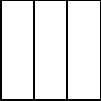
\includegraphics[scale=1]{taskbook-98}
\\[2pt]
\hspace{1pt} 
Draufsicht
\hspace{43pt} Frontalansicht
\end{figure}
\newline\quad
{\bf 15.} Wie viele verschiedene Arten gibt es, die Nummer 64 in zehn ganze, positive Zahlen zu zerlegen, wovon keine grösser als 12 ist?
%\newline
[Antworten, die sich nur in der Reihenfolge der Zahlen unterscheiden, gelten als gleich.]
\newline\newline\quad
{\bf 16.} Wenn man gleichlange Stäbe (wie z.B. Dominosteine) übereinander legt, wird einen Überhang der Länge $x$ geschaffen. Was ist die maximale Länge des Überhanges, die man so erstellen kann? 
\begin{figure}[h!]
\centering
\footnotesize
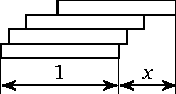
\includegraphics[scale=1]{taskbook-97}
\end{figure}
%\newline\newline\quad
\begin{figure}[h]
\begin{minipage}[c][][c]{0.7 \textwidth}
{\bf 17.} Die Entfernung zwischen den Städten $A$ und $B$ beträgt 40 km. Zwei Fahrradfahrer verlassen gleichzeitig jeweils $A$ und $B$ und fahren sich direkt entgegen, einer mit 10 km/h und der andere mit 15 km/h. Eine Fliege fliegt mit dem ersten Radfahrer von $A$ los mit einer Geschwindigkeit von 100 km/h, erreicht den zweiten Radfahrer, berührt seine Stirn und fliegt dann zurück zur Stirn des ersten Radfahrers, dann wieder zurück zum zweiten und so weiter bis die beiden Köpfe der Radfahrer zusammenstossen und die Fliege zwischen ihre Stirne zerkwetschen. 
Wie viele Kilometer ist die Fliege im ganzen geflogen? 
\end{minipage}
\hfill
\begin{minipage}[c]{0.2 \textwidth}
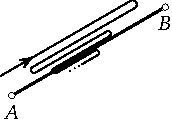
\includegraphics[scale=1]{taskbook-1}
\end{minipage}
\end{figure}

\medskip\noindent
{\bf 18.} Ein Dominostein verdeckt zwei Felder eines Schachbretts. Mit nur 31 Dominosteinen, verdecke das ganze Schachbrett mit aussnahme von zwei gegenüberliegenden Eckfeldern. [Ein Schachbrett besteht aus $8 \times 8 = 64$ quadratischen Feldern.]
\begin{figure}[h]
\centering
\footnotesize
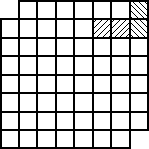
\includegraphics[scale=1]{taskbook-2}
\end{figure}

\noindent{\bf 19.} Eine Raupe in einem Quader-förmigen Raum möchte von der Ecke links unten am Boden und zur gegenüberliegenden Ecke, oben rechts an der Decke, gelangen. 
Finde die kürzest-mögliche Bahn für die Raupe entlang der Wände. 
\begin{figure}[h]
\centering
\footnotesize
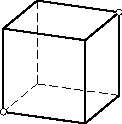
\includegraphics[scale=1]{taskbook-3}
\end{figure}
\newline\newline\quad
{\bf 20.} Du hast Wasser aus dem Wasserhahn und zwei Behälter, einer mit 5 Liter Volumen und einer mit 3 Liter Volumen. Wie kannst du einen Liter in einem der Gefäße erhalten?
\begin{figure}[h!]
\centering
\footnotesize
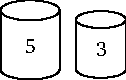
\includegraphics[scale=1]{taskbook-4}
\end{figure}

%\newline\newline\quad
\medskip\noindent
{\bf 21.} In einer Familie sind fünf Köpfe und vierzehn Beine. Wie viele Menschen und wie viele Hunde sind in der Familie?
%\newline\quad
\begin{figure}[h!]
\begin{minipage}[c][][c]{0.7 \textwidth}
{\bf 22.} Gleichseitige Dreiecke werden nach aussen auf den Seiten $AB$, $BC$ und $CA$ des Dreiecks $ABC$ konstruiert. Beweise dass die Zentren ($*$) der Dreiecke ein gleichseitiges Dreieck bilden.\end{minipage}
\hfill
\begin{minipage}[c]{0.2 \textwidth}
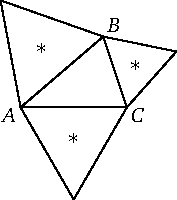
\includegraphics[scale=1]{taskbook-6}
\end{minipage}
\end{figure}

\newpage
\noindent
{\bf 23.} Welche Vielecke können durch den Schnitt eines Würfels mit einer Ebene entstehen? Kann ein Fünfeck, ein Siebeneck oder gar ein regelmäßiges Sechseck entstehen? 
\begin{figure}[h]
\centering
\footnotesize
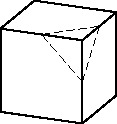
\includegraphics[scale=1]{taskbook-7}
\end{figure}
\newline\newline\quad
{\bf 24.} Zeichne eine Gerade durch die Mitte eines Würfels, so dass die Summe der Quadrate der Entfernungen zwischen ihr und den acht Eckpunkten des Würfels (im Vergleich zu andern Geraden durch die Mitte) möglichst a) gross, b) klein ist.
\newline\newline\quad
{\bf 25.} Ein gerader kreisförmiger Kegel wird von einer Ebene so geschnitten, dass eine geschlossene Kurve entsteht. Zwei Kugeln sind dem Kegel so eingeschrieben, dass sie die Ebene berühren, eine in Punkt $A$ und die andere in Punkt $B$. Finde den Punkt $C$ auf der Schnittkurve, um die Summe der Distanzen $CA + CB$ möglichst a) gross b) klein zu machen. 
\begin{figure}[h]
\centering
\footnotesize
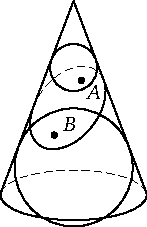
\includegraphics[scale=1]{taskbook-9}
\end{figure} 
\newline\newline\quad {\bf 26.} Die Erdoberfläche wird auf einen Zylinder projiziert. Der Mantel dieses Zylinders wird durch die Tangenten zu den Längengraden am Äquator geformt. Was ist grösser: die tatsächliche Fläche Frankreichs oder die projizierte Fläche?

\begin{figure}[h]
\centering
\footnotesize
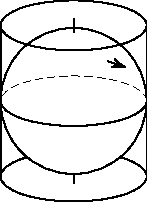
\includegraphics[scale=1]{taskbook-10}
\end{figure}

\newpage
\noindent
{\bf 27.} Beweise, dass wenn die Zahl $2^{p-1}$ durch eine ungerade Primzahl $p$ geteilt wird, der Rest 1 sein muss. (Beispiele: $2^2 = 3a +1,$ $2^4 = 5b+1,$ $2^6 = 7c+1,$ 

$2^{10} - 1 = 1023 = 11\cdot 93$). 
\newline\newline\quad
{\bf 28.} Eine 10 cm lange Nadel wird willkürlich auf eine linierte Seite Papier geworfen dessen Linienabstand ebenfalls 10 cm ist. Dieser Vorgang wird $N$ (eine Million) mal wiederholt. 
Ungefähr wie oft wird die Nadel eine Linie kreuzen? 
\begin{figure}[h]
\centering
\footnotesize
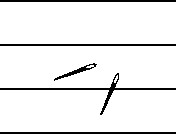
\includegraphics[scale=1]{taskbook-12}
\end{figure}

Es ist möglich, dieses Experiment mit nur $N=100$ auszuführen (wie ich es mit 10 Jahren tat) anstatt einer Million. [Die Antwort dieser Frage ist überraschend: $\frac2{\pi}N$. Ausserdem, wenn die Nadel gekrümmt ist mit einer Länge $a \cdot 10$ cm, ist die Antwort mit $N$ Würfen annäherungsweise $\frac{2a}{\pi}N$. 
Die Zahl $\pi \approx \frac{355}{113} \approx \frac{22}7.$]
\newline\newline\quad
{\bf 29.} Jene Polyeder, in denen alle Seitenflächen identisch sind, nennt man Platonische Körper. Manche unter ihnen haben dreieckige Seitenflächen: Tetraeder (4 Seitenflächen), Oktaeder (8 Seitenflächen), Ikosaeder (20 Seitenflächen, 12 Ecken und 30 Kanten; dieses ist interessant zu zeichnen.). 
\begin{figure}[h!]
\centering
\footnotesize
\hspace{5pt}
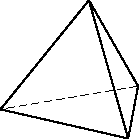
\includegraphics[scale=1]{taskbook-131}\hspace{68pt}
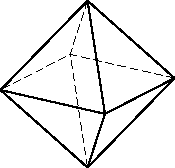
\includegraphics[scale=1]{taskbook-132}\\ \vspace{3pt}
Tetraeder (tetra${}= 4$) \hspace{40pt}
Oktaeder (octo${}= 8$)\\[25pt]
{\Huge 
%{}\hskip20pt 
?}\\ Ikosaeder\vspace{3pt}
\end{figure}
%\newline\quad
Überprüfe die folgende Behauptung: Die Anzahl der Seitenflächen eines konvexen Polyeders mit dreieckigen Seitenflächen gleicht zweimal der Anzahl der Ecken minus vier. 
\newpage
\noindent
%\newline\newline\quad
{\bf Noch ein platonischer Körper (es gibt fünf insgesamt)}
\begin{figure}[h]
\centering
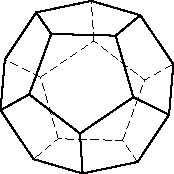
\includegraphics{taskbook-14}\\[2pt]
\end{figure}

\noindent
{\bf 30.} Ein Dodekaeder ist ein konvexes Polyeder mit zwölf identischen regelmäßigen fünfeckigen Seitenflächen. Es hat zwanzig Ecken und dreißig Kanten (Im Übrigen befinden sich die Ecken des Dodekaeders jeweils in der Mitte der Seitenflächen eines Ikosaeders).
Finde fünf Würfel die in den Dodekaeder so passen, dass ihre Ecken auch Ecken des Dodekaeders sind und ihre Kanten Diagonalen der Seitenflächen des Dodekaeders sind (ein Würfel hat 12 Kanten, eine pro Seitenfläche (?????)). [Diese Frage wurde von Johannes Kepler erfunden, um Planetenbahnen zu beschreiben.]
\bigskip
\noindent{\bf 31.} Beschreibe das Schnittvolumen von zwei Tetraedern, die in einen Würfel passen, so dass ihre Ecken auch Ecken des Würfels sind und ihre Kanten Diagonalen der Seitenflächen. 
Welcher Bruchteil des Würfel-Volumens stellt dieser Schnitt dar?
\newline\newline\quad
$\mathbf 31^{bis}.$ 
Konstruire den Schnitt zwischen einen Würfel und einer Ebene, die durch drei gegebene Punkte auf den Würfelkanten geht. [Zeichne das Vieleck, welches die Schnittfläche der beiden Körper bildet.]
\begin{figure}[h]
\centering
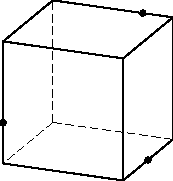
\includegraphics{taskbook-15}
\end{figure}

\noindent{\bf 32.} Wie viele Symmetrien hat ein Tetraeder? Wie viele hat ein Würfel? Ein Oktaeder ? Ein Ikosaeder ? Ein Dodekaeder? Eine Symmetrie ist eine Umwandlung, die ein Objekt auf sich selbst abbildet, also auch die Längen des Objektes beibehält. 
Wie viele davon sind Drehsymmetrien und wie viele davon sind Spiegelsymmetrien ?
\bigskip
\noindent{\bf 33.} Wie viele verschiedene Arten gibt es, einen Würfel mit 6 verschiedenen Farben (1, ...6) [eine pro Seite] anzumalen? Würfel die sich nur durch eine Rotation unterscheiden gelten hier als gleich.
\begin{figure}[h]
\centering
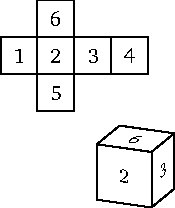
\includegraphics{taskbook-17}
\end{figure}

\noindent{\bf 34.} In wie vielen verschiedenen Arten können $n$ Objekte angeordnet werden? 
Für drei Objekte zum Beispiel gibt es sechs verschiedene Anordnungen: $n=3$: (1,2,3), (1,3,2), (2,1,3), (2,3,1), (3,1,2), (3,2,1). 
Wie viele Anordnungen gibt es für $n=4$? $n=5$? $n=6$? $n=10$?
\begin{figure}[h]
\centering
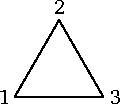
\includegraphics{taskbook-18}
\end{figure}

\noindent{\bf 35.} Ein Würfel hat 4 lange Diagonalen. Wie viele Permutationen dieser Diagonalen können durch die Rotation eines Würfels erhalten werden?
\begin{figure}[h]
\centering
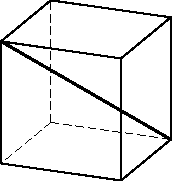
\includegraphics{taskbook-19}
\end{figure}

\noindent{\bf 36.} Ist die Differenz zwischen der Summe der Kubik dreier Zahlen und der Kubik der Summe dieser drei Zahlen immer durch 3 teilbar? 

\bigskip
\noindent{\bf 37.} Lösen sie Frage Nummer 36, aber für die fünfte Potenz und Teilbarkeit durch fünf, und für die siebte Potenz und Teilbarkeit durch 7. 

\bigskip
\noindent{\bf 38.} Finde diese Summe:
$${1 \over 1\cdot 2} + {1 \over 2\cdot 3} + {1 \over 3\cdot 4} + \dots + {1 \over 99\cdot 100}$$
(mit einer Fehlerschranke nicht grösser als $1\%$ der Antwort).

\bigskip
\noindent{\bf 39.} Zwei verschiedene Vielecke mit derselben Fläche können in eine begrenzte Anzahl von kleineren Vielecken geteilt werden, so dass aus diesen Teilen beide Vielecke geformt werden können. Beweise dieses! [Dieser Satz stimmt nicht für dreidimensionale Körper: Ein Würfel und ein Tetraeder mit gleichem Volumen können nicht in dieser Weise unterteilt werden!]
\begin{figure}[h]
\centering
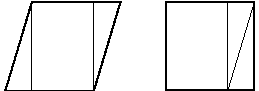
\includegraphics{q39_horizontal}\\[6pt]
\end{figure}

\noindent{\bf 40.} Ein Parallelogramm wird auf kariertem Papier so gezeichnet, dass seine Ecken auf Ecken der Karos liegen und so, dass weder auf den Kanten noch innerhalb der Figur weitere Karo-Ecken liegen. Beweise dass der Flächeninhalt dieses Parallelogramms der Fläche eines der Karos gleicht. 
\begin{figure}[h]
\centering
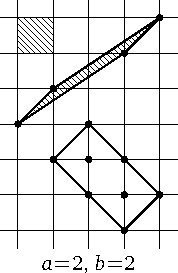
\includegraphics{taskbook-24}\vskip3pt
\end{figure}

\medskip
\noindent{\bf 41.} Nehme die selben Voraussetzungen an wie in Frage 40, nur dass $a$ Ecken innerhalb des Parallelogramms liegen und $b$ Ecken auf den Kanten. Finde die Fläche dieses Parallelogramms.

\bigskip
\noindent{\bf 42.} Gilt die entsprechende Fassung der Aussage in Frage 40 auch für ein drei dimensionales Parallelepiped?

\bigskip
\noindent{\bf 43.} Die Fibonacci-Zahlen formen die folgende Folge $(a_1=1)$, $1$, $2$, $3$, $5$, $8$, $13$, $21$,
$34$,\nobreak\ $\dots$, wo $a_{n+2}=a_{n+1}+a_n$ für alle
$n=1$, $2$,\nobreak\ $\dots$ \ . Finde den größten gemeinsamen Teiler der Zahlen $a_{100}$ und $a_{99}$.

\newpage
%\bigskip
\noindent{\bf 44.} Finde die Anzahl (Catalan-Zahl) der verschiedenen Dreieckszerlegungen eines konvexen n-ecks durch seine sich nicht schneidenden Diagonalen.
Zum Beispiel, $c(4)=2$, $c(5)=5$, $c(6)=14$. Wie kann man $c(10)$ bestimmen ?

\begin{figure}[h]
\centering
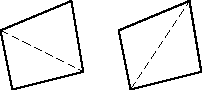
\includegraphics[scale=1]{taskbook-281}
\hskip1cm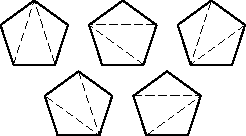
\includegraphics[scale=1]{taskbook-282}
\end{figure}


%\newpage
\noindent{\bf 45.} Ein Turnier hat $n$ Mannschaften. Wenn eine Mannschaft verliert, scheidet sie aus dem Turnier. Der Sieger wird also durch $n-1$ Partien entschieden. 
Der Ablaufplan kann symbolisch so notiert warden: $((a,(b,c)),d)$ welches bedeutet dass $b$ zuerst $c$ trifft, der Sieger dann $a$ trifft, und der Sieger dieser Partie trifft dann $d$. 
Was ist die Anzahl von unterschiedlichen Ablaufplänen für 10 Mannschaften?

Für 2 Mannschaften gibt es nur eine Möglichkeit $(a,b)$. Die Anzahl ist 1.
Für 3 Mannschaften gibt es nur $((a,b),c)$, oder $((a,c),b)$, oder $((b,c),a)$. Die Anzahl ist also 3.

Für 4 Mannschaften gibt es die folgenden Ablaufpläne:

$$\begin{array}{cccc}
(((a,b),c),d) & \quad (((a,c),b),d) & \quad (((a,d),b),c) & \quad (((b,c),a),d) \\
(((b,d),a),c) & \quad (((c,d),a),b) & \quad (((a,b),d),c) & \quad (((a,c),d),b) \\ 
(((a,d),c),b) & \quad (((b,c),d),a) & \quad (((b,d),c),a) & \quad (((c,d),b),a) \\
((a,b),(c,d)) & \quad ((a,c),(b,d)) & \quad ((a,d),(b,c))

\end{array}$$

\bigskip
\noindent{\bf 46.} Verbinde die $n$ Punkte $1, 2, \dots, n$ mit $n-1$ linien. Wie viele verschiedene Bäume können so erhalten werden (der Fall $n=5$ ist schon sehr interessant!)?
\medskip
$n=2$:\quad 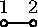
\includegraphics{taskbook-291}\,,\quad die Anzahl ist 1; 

\medskip
$n=3$:\quad 
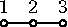
\includegraphics{taskbook-292}\,,\quad 
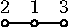
\includegraphics{taskbook-293}\,,\quad 
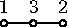
\includegraphics{taskbook-294}\,,\quad 
die Anzahl ist 3;

\medskip
$n=4$:\quad\def\quad{\hskip.7em}
$\vcenter{\hbox{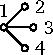
\includegraphics{taskbook-295}}}$,\quad
$\vcenter{\hbox{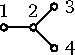
\includegraphics{taskbook-296}}}$,\quad
$\vcenter{\hbox{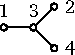
\includegraphics{taskbook-297}}}$,\quad
$\vcenter{\hbox{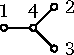
\includegraphics{taskbook-298}}}$,\quad
$\vcenter{\hbox{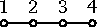
\includegraphics{taskbook-299}}\hbox{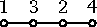
\includegraphics{taskbook-290}}
\vskip-8pt
\hbox to50bp{\dotfill}}$,\quad 
die Anzahl ist 16.


\newpage
\noindent{\bf 47.} Eine Permutation $(x_1,x_2, \dots,x_n)$ von den Zahlen $\{1, 2, \dots, n\}$ wird eine
\emph{Schlange} mit Länge $n$ genannt wenn $x_1<x_2>x_3<x_4 \dots$ \ .
\medskip

{\sc Example.}
$\begin{aligned}[t]
&\begin{aligned}[t] n=2, \text{ only } 1<2, \end{aligned} &&\text{die Anzahl von Schlangen ist }1, \\
&\hskip-\nulldelimiterspace\mathord{\left.\begin{aligned} n=3, \hphantom{\text{ only }} 1&<3>2 \\ 
2&<3>1\end{aligned} \right\}}, && \text{die Anzahl von Schlangen ist }2, \\[2pt]
&\hskip-\nulldelimiterspace\mathord{\left.\begin{aligned} n=4, \hphantom{\text{ only }} 1&<3>2<4 \\ 
1&<4>2<3 \\ 
2&<3>1<4 \\ 
2&<4>1<3 \\ 
3&<4>1<2\end{aligned} \right\}},
&&\text{die Anzahl von Schlangen ist }5. \\
\end{aligned}$

\medskip
\noindent 
Finde die Anzahl von Schlangen mit Länge 10. 

\bigskip
\noindent{\bf 48.} Sei $s_n$ die Anzahl von Schlangen mit Länge $n$:
$$
s_1=1, \quad s_2=1, \quad s_3=2, \quad s_4=5, \quad s_5=16, \quad s_6=61.
$$
Beweise, dass die Taylorreihe des Tangens ist wie folgt: 
$$
\tan x=1\, \frac{x^1}{1!}+2\, \frac{x^3}{3!}+16\, \frac{x^5}{5!}+\dots=
\textstyle\sum\limits_{k=1}^{\infty} s_{2k-1}\, \frac{x^{2k-1}}{(2k-1)!}.
$$

\bigskip
\noindent{\bf 49.} Finde die Summe dieser Reihe.
$$
1+1\, \frac{x^2}{2!}+5\, \frac{x^4}{4!}+61\, \frac{x^6}{6!}+\dots=
\textstyle\sum\limits_{k=0}^{\infty} s_{2k}\,\frac{x^{2k}}{(2k)!}.
$$

\bigskip
\noindent{\bf 50.} Für $s>1$, beweise folgende Gleichung:
$$
\textstyle\prod\limits_{p=2}^{\infty} \cfrac{1}{1-\cfrac{1}{p^s}}=\sum\limits_{n=1}^{\infty} \frac{1}{n^s}
$$ 
(Das Produkt ist über alle Primzahlen $p$. Die Summe ist über alle natürliche Zahlen~$n$).

\newpage
%\bigskip
\noindent{\bf 51.} Finde die Summe dieser Reihe:
$$
1+ \frac{1}{4}+ \frac{1}{9}+\dots=\textstyle\sum\limits_{n=1}^{\infty} \frac{1}{n^2}
$$
(beweise, dass die Antwort $\pi^2/6$, ist, also schätzungsweise $3/2$). 

\bigskip
\noindent{\bf 52.} Finde die Wahrscheinlichkeit, das der Bruch $p/q$ in gekürzter Form vorliegt. $p$ und $q$ sind in diesem Fall durch die Kreisscheibe $p^2+q^2 \leqslant R^2$ definiert. Wir zählen die Anzahl $N$ der Vektoren mit ganzen Zahlen $p$ und $q$, welche keinen gemeinsamen Teiler größer als 1 haben. Die Wahrscheinlichkeit, das der Bruch $p/q$ nicht gekürzt werden kann, ist dann der Grenzwert des Bruches $N(R)/M(R)$, wobei $M(R)$ die Anzahl der ganz-zähligen Punkte in der Kreisscheibe ist $(M \sim \pi R^2)$).
\begin{figure}[h]
\footnotesize
\centering
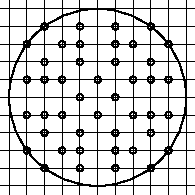
\includegraphics{taskbook-36}\\{\ } \\
$M(5)=81$, $N(5)=44$, $N/M = 44/81$
\end{figure}

\bigskip
\noindent{\bf 53.} Finde den Grenzwert des Quotients $a_{n+1}/a_n$ für die Fibonacci Zahlen $a_n$ von Aufgabe 43, wenn $n$ gegen unendlich geht: 
\vspace{2\jot}
\[
\frac{a_{n+1}}{a_n}=2,\ \frac 32,\ \frac53, \ \frac85, \ \frac{13}8,
\ \frac{34}{21}.
\vspace{\jot}
\] 

%\noindent
\textsc{Antwort:} "Der Goldene Schnitt",
$\frac{\sqrt{5}+1}{2\vphantom)} \approx 1{,}618$. [Dieses ist das Teilungsverhältnis der zwei Längen eines Rechtecks $ABCD$ dass selbstähnlich mit dem Rest ist, den man erhält, wenn man das Quadrat $ABPQ$ davon abschneidet: 
$\frac{AB}{BC}=\frac{PC}{CD\vphantom)}$.] Was hat der goldene Schnitt mit einem regelmäßigen Fünfeck und einem Pentagramm (fünf-zackiger Stern) zu tun?

\begin{figure}[h]
\centering
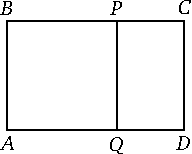
\includegraphics{taskbook-37}
\end{figure}

\newpage
%\medskip
\noindent{\bf 54.} Bestimme den Grenzwert des unendlichen Kettenbruches:
\begin{align*}
1+\cfrac{1}{2+\cfrac{1}{1+\cfrac{1}{2+\cfrac{1}{1+\cfrac{1}{2+\ldots}}}}}=
a_0+\cfrac{1}{a_1+\cfrac{1}{a_2+\cfrac{1}{a_3+\dots}}} \qquad
\smash{
%\medmath
{\left[\begin{aligned} &a_{2k}=1 \\[-\jot] &a_{2k+1}
=2 \end{aligned}\right]} }
\end{align*}

\medskip

\noindent (in anderen Worten, bestimme den Grenzwert des folgenden Bruches:
$$
a_0+\cfrac{1}{a_1+\cfrac{1}{a_2+{\atop{\ddots \atop {}} + \cfrac{1}{a_n}}
} 
}
$$
für $n \to \infty$).


\bigskip
\noindent{\bf 55.} Bestimme die Polynome 
\[
y=\cos 3 (\arccos x),\ y=\cos 4 (\arccos x),\ 
y=\cos n (\arccos x),
\] 
wo $|x| \leqslant 1$. 


\bigskip
\noindent{\bf 56.} Bestimme die Summe der $k$-ten Potenz der $n$-ten Einheitswurzeln.

\bigskip
\noindent{\bf 57.} In einem Koordinaten-Diagramm, zeichne die Kurven der folgenden Gleichungen in Parameterdarstellung: 
\[
\{x=\cos 2t, y=\sin 3t\},\quad 
\{x=t^3-3t, y=t^4-2t^2\}.
\]

\bigskip
\noindent{\bf 58.} Bestimme (mit einer Fehlerschranke nicht grösser als 10\% der Antwort)
$$
\int\limits_0^{2\pi} \sin^{100} x\,dx.
$$

\bigskip
\noindent{\bf 59.} 
Bestimme (mit einer Fehlerschranke nicht grösser als 10\% der Antwort)
$$
\int\limits_1^{10} x^x\,dx.
$$

\bigskip
\noindent{\bf 60.} Bestimme die Fläche eines Dreiecks mit Winkeln $(\alpha, \beta, \gamma)$ auf einer Kugel mit Radius 1, wobei die Seiten des Dreiecks auf Grosskreisen liegen (Schnitte einer Kugel mit Ebenen, welche die Mitte der Kugel enthalten).

\medskip
%\noindent
\textsc{Antwort:} $S=\alpha+\beta+\gamma-\pi$ (zum Beispiel, für ein Dreieck mit drei rechten Winkeln, $S=\pi/2$, in diesem Fall ist die Fläche ein achtel der Gesamtfläche der Kugel).
\begin{figure}[h]
\centering
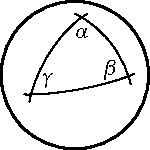
\includegraphics{taskbook-44}\hskip2cm 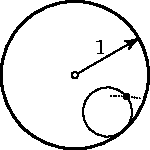
\includegraphics{taskbook-45}
\end{figure}

\bigskip
\noindent{\bf 61.} Ein Kreis mit Radius $r$ rollt (ohne zu rutschen) innerhalb eines Kreises mit Radius 1 ab.
Zeichne die vollständige Bahn eines Punktes auf dem rollenden Kreis für $r=1/3$, für $r=1/4$, für $r=1/n$, und für $r=1/2$. (Solche Bahnen nennen sich Hypozykloide)

\bigskip
\noindent{\bf 62.} Für eine Klasse mit $n$ Schülern, schätze die Wahrscheinlichkeit, dass zwei Schüler am gleichen Tag Geburtstag haben. Ist sie hoch oder niedrig? 

%\noindent
\medskip
(Finde die Wahrscheinlichkeit dass $p \approx 1/2$ ist).

\bigskip
\noindent{\bf 63.} Das Snelliussche Brechungsgesetz besagt, dass der Winkel $\alpha$ zwischen einem Lichtstrahl und der Senkrechten zu den Schichten eines mehrschichtigen Mediums durch die folgende Gleichung bestimmt wird: $n(y) \sin \alpha=\text{const}$,
wobei $n(y)$ der refractive Index einer Schicht der Höhe $y$ ist (der Index $n$ ist umgekehrt proportional zu der Lichtgeschwindigkeit im Medium, wenn die Geschwindigkeit im Vakuum als 1 angenommen wird; in  Wasser ist er $n=4/3$).
\begin{figure}[h]
\centering
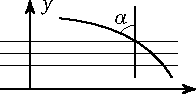
\includegraphics{taskbook-47}\hskip2cm
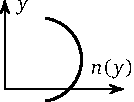
\includegraphics{taskbook-471}
\end{figure}

%\noindent 
Zeichne die Bahnen von Lichtstrahlen im Medium “Luft über eine Wüste”, wobei der Index $n(y)$ bei einer bestimmten Höhe sein Maximum erreicht (eine Lösung zu dieser Frage erklärt die Erscheinung einer Fata Morgana in der Wüste).

\newpage
\noindent{\bf 64.} Schreibe das Dreieck $KLM$ mit dem kleinstmöglichen Umfang in das spitzwinklige Dreieck $ABC$ ein (Ecke $K$ ist auf $AB$, $L$ auf $BC$, $M$ auf $CA$).
\begin{figure}[h]
\centering
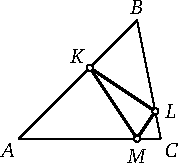
\includegraphics{taskbook-48} 
\end{figure}

\textsc{Hinweis:} Die Antwort für nicht-spitzwinklige Dreiecke ist nicht der schönen Antwort für spitzwinklige Dreiecke ähnlich. 

\bigskip
\noindent{\bf 65.} 
Berrechne den Mittelwert der Funktion $1/r$ (wobei $r^2\,=x^2\,+y^2+z^2$, $r$ ist der Abstand zum Ursprung)  auf der Kugel mit Radius $R$ und Mittelpunkt $(X,Y,Z)$.

%\noindent
\medskip
\textsc{Hinweis:} Dieses Problem ist dem Newtonschen Gravitationsgesetz und dem Colombschen Gesetz für Elektrizitätstheorie verwandt. In der zweidimensionalen Version dieses Problems ist die Funktion durch $\ln r$ zu ersetzen, und die Kugel durch einen Kreis.


\bigskip
\noindent{\bf 66.} Aus der Tatsache dass $2^{10}=1024 \approx 10^3$ kann man schlussfolgern dass $\log_{10} 2 \approx 0{.}3$.

Schätze den Unterschied zwischen $\log_{10} 2$ und $0{.}3$ und berrechne $\log_{10} 2$ auf drei Dezimalstellen genau. 

%{\addfontfeature{WordSpace={.97,1,1},LetterSpace=0}
\bigskip
\noindent{\bf 67.} Bestimme $\log_{10} 4$, $\log_{10} 8$,
$\log_{10} 5$, $\log_{10} 50$, $\log_{10} 32$, $\log_{10} 128$,
$\log_{10} 125$, $\log_{10} 64$ mit der gleichen Genauigkeit.

\bigskip
\noindent{\bf 68.} Gegeben dass $7^2 \approx 50$ ist, schätze den Wert von $\log_{10} 7$. 

\bigskip
\noindent{\bf 69.} Bestimme $\log_{10} 9$, $\log_{10} 3$,
$\log_{10} 27$, $\log_{10} 6$, $\log_{10} 12$, wobei $\log_{10} 64$ und $\log_{10} 7$ gegeben sind.

\bigskip
\noindent{\bf 70.} Gegeben sei dass $\ln (1+x) \approx x$ ($\ln$ is $\log_e$). Bestimme daher den Wert für $\log_{10} e$ und $\ln 10$ mit Hilfe der Gleichung \footnote{
%\addfontfeature{LetterSpace=-1}
Die Eulerzahl $e = 2{,}71828\dots$ ist definiert als der Grenzwert der Folge $\left(1+\frac1n\right)^n$ für $n\to \infty$, und ist gleich der Summe der Reihe 
$1+\frac 1{1!} +\frac 1{2!}+\frac 1{3!}+\dots$. Sie kann auch anhand der Formel für $\ln (1+x)$: $\lim\limits_{x\to 0}\frac{\ln(1+x)}{x} = 1$ definiert werden.}\vspace{-\jot}
%
$$
\log_{10} a=\frac{\ln a}{\ln 10}
$$ 
und der Werte für $\log_{10} a$ die vorher berechnet wurden (zum Beispiel, für $a=128/125$, $1024/1000$ und so weiter).

%\noindent
[Antworten zu den Aufgaben 65--69 geben eine Tabelle für 4-stellige Logarithmen von irgendeiner Zahl, mit Hilfe der Produkte von Zahlen die im voraus als Grunddaten bestimmt wurden, sowie der Formel: 
\vspace{-2\jot}
\[
\ln (1+x) \approx x-\frac{x^2}{2}+\frac{x^3}{3}-\frac{x^4}{4}+\dots
\]
für Fehlerbehebnisse.] (In dieser Weise stellte Newton eine Tabelle von 40-stelligen Logarithmen zusammen!)

\bigskip
\noindent{\bf 71.} Bedenke die Folge der Zweier-Potenzen: $1$, $2$, $4$, $8$, $16$, $32$, $64$, $128$, $256$, $512$, $1024$, $2048, \dots$ . In den ersten zwölf Zahlen fangen vier davon mit 1 an, und gar keine mit 7. 

%\noindent 
Beweise, dass für den Grenzwert $n \to \infty$, die erste Ziffer der Zahlen $2^m$,
$0\leqslant m \leqslant n$, mit einer bestimmten Frequenz aufkommen: 
$p_1 \approx 30\%$, $p_2 \approx 18\%$, $\dots$, $p_9 \approx 4\%$.

\bigskip
\noindent{\bf 72.} Bedenke die erste Ziffer der Dreier-Potenzen: $1$,
$3$, $9$, $2$, $8$, $2$, $7, \dots$ . Beweise, dass für den gleichen Grenzwert ebenfalls bestimmte Frequenzen aufkommen, und zwar die gleichen wie für die Zweier-Potenzen. Finde die genauen Werte für $p_1, \dots, p_9$.

%\noindent
\medskip
\textsc{Hinweis:} Die erste Ziffer einer Zahl $x$ ist durch den Dezimalteil der Zahl 
$\log_{10} x$ bestimmt, also hat man den Dezimalteil der Zahlen $m \alpha$ zu betrachten, wobei $\alpha=\log_{10} 2$.

%\noindent 
Beweise dass dieser Dezimalteil über das Intervall von 0 zu 1 gleichmäßig verteilt ist:  aus den $n$ Dezimalteilen der Zahlen $m \alpha$, $0 \leqslant m<n$, wird ein Subinterval $A$  die Anteil ~$k_n (A)$ enthalten, so dass, für $n \to \infty$,
$\lim (k_n (A)/n)={}$(Die Länge des Subintervals~$A$).
\pagebreak[3]

\bigskip
\noindent{\bf 73.} Sei $g\colon M \to M$ eine nahtlose Abbildung des begrentzten Definitionsbereich $M$ auf sich selbst, welche eins-zu-eins ist und die Fläche des Definitionsbereich erhält (Volumen im Multi-dimensionalen Fall).

My contribution: (???) Sei $g\colon M \to M$ eine glatte, injektive Abbildung von dem beschränktes Gebiet $M$ auf sich selbst die ....

%\noindent 
Beweise, dass in der Nähe $U$ von jedem beliebigen Punkt von $M$ und für beliebige $N$ ein Punkt $x$ existiert, so dass $g^T x$ auch in $U$ liegt für bestimmte ganze Zahlen $T>N$ (``Das Rekurrenz-Theorem").
??? My Version:
Beweise dass zu jedem Punkt in $M$, zu jeder Umgebungen $U$ dieses Punktes und für alle $N$ es ganze Zahlen $T>N$ gibt, für die gilt dass $g^T x$ sich auch in $U$ gefindet. ("poincarésche Wiederkehrsatz").

\bigskip
\noindent{\bf 74.} Sei $M$ die Torusoberfläche (mit Koordinaten $\alpha$ (mod $2\pi$), $\beta$ (mod $2\pi$)) und $g(\alpha, \beta)=(\alpha+1, \beta+ \sqrt{2})$ (mod $2\pi$). Beweise dass die Folge von Punkten $\{g^T (x)\}$, $T=1, 2, \dots$ überall in dem Torus dicht liegt.

\bigskip
\noindent{\bf 75.} Sei nun, in Bezug auf Aufgabe 74, 
$$
g(\alpha, \beta)=(2\alpha+\beta,\alpha+\beta) \pmod {2\pi}.
$$ 
Beweise die Existenz einer überall dichten Untermenge, die aus periodischen Punkten $x$ des Torus' besteht (das heisst, es gilt $g^{T (x)} x=x$ für gewisse ganze Zahlen $T>0$).

\bigskip
\noindent{\bf 76.} In Bezug auf Aufgabe 74, beweise dass für fast alle Punkte $x$ auf dem Torus, die Folge der Punkte $\{g^T (x)\}$, $T=1, 2, \dots$ überall auf dem Torus dicht ist (Punkte $x$ ohne diese Eigenschaft bilden eine Menge der Grösse null). 

\bigskip
\noindent{\bf 77.} In Bezug auf Aufgaben 74 und 76, beweise dass die Folge $\{g^T (x)\}$, $T=1, 2, \dots$ über den Torus gleichförmig (uniform) verteilt ist: wenn sich $k_n(A)$ aus den $n$ Punkten in dem Definitionsbereich $A$ befinden, mit $T=1, 2, \dots,n$, dann
$$
\lim_{n \to \infty} \frac{k_n(A)}{n}=\frac{\operatorname{mes} A}{\operatorname{mes} M}
$$
(zum Beispiel, für einen Jordan-messbaren Definitionsbereich $A$ mit Maß $\operatorname{mes} A$).

\ 

\ 

\ 

\textsc{Anmerkung zu Aufgabe 13.} Ich habe in meinem Beitrag zur Weihnacht-Jubiläums-Ausgabe im Jahr 2000 der Zeitschrift ''Physics—Uspekhi'' versucht, anhand dieser Aufgabe die unterschiedlichen Herangehensweisen darzustellen, die man typischer Weise bei Mathematikern und Physikern findet. Mein Erfolg übertraf meine Erwartungen: die Redaktion, ungleich zu Vorschülern, konnte dieses Problem nicht lösen, und änderte dann meine 4 mm Antwort wie folgt: anstatt ''von der ersten Seite im Band 1 bis zur letzten Seite im Band 2'' hieß es in der Veröffentlichung ''von der {\em letzen\/} Seite im Band 1 bis zur {\em ersten\/} Seite im Band 2''. 

Diese wahre Geschichte ist so unglaublich, dass ich sie hier erwähne: der Beweis ist die Erstveröffentlichung von der Redaktion. 
\ 

\vspace{0pt plus 12pt}
\centerline{*\quad *\quad*}
\vspace{.4\baselineskip}

\

\ 

\ 

{\em
\rightline{
\begin{tabular}{l}
Translated by \\
Victor Goryunov and Sabir Gusein-Zade \\
from the original Russian edition: \\
Moscow, MCCME, 2004 \\
ISBN 5-94057-183-2\\
\\
Picture credits title page:\\
Archives of the 
Mathematisches \\Forschungsinstitut Oberwolfach.
\end{tabular}
}
}
\end{document}
